\scanpage{25}
% archive foliation: 24
\diagram{\begin{tikzcd}
\operatorname{Ker}i\arrow[r,dashed]\arrow[d]&L\arrow[dl,dashed]&\\
J&L'\arrow[l,dashed]\arrow[u,dashed,"\unsure{\alpha}"]&M'\arrow[l,dashed]\\
&&\operatorname{Ker}\beta\arrow[u,dashed]\arrow[ull]
\end{tikzcd}}
\margin{\figure{\begin{tikzpicture}
\node[anchor=north west,inner sep=0,text width=7cm,align=left] at (0,0) {\diagram{\begin{tikzcd}[ampersand replacement=\&]
L+M'\arrow[r,two heads,"(i,\beta)","\text{surj}"'{draw,rounded corners=8pt,inner sep=1pt}]\arrow[d,"(\sigma,\sigma\alpha\pi')=\rho"']\&M\arrow[ddl,dashed,"\mu"]\\
J\arrow[d,"\lambda"']\&\\G\&
\end{tikzcd}}
Condition de non ramification.
Le foncteur en $G$ est repr. par $\operatorname{Coker}\rho$, dont la
formation commute à tout chgt de base.};
\draw (-0.25,0.3)--(-0.25,-3.7)..controls(-0.25,-4.1)and(0.7,-4)..(0.85,-4.4)..controls(0.9,-4.7)and(1.3,-4.6)..(1.7,-4.6)--(5.6,-4.6)..controls(6,-4.6)and(6,-4.95)..(6.6,-4.95)--(7.05,-4.9);
\end{tikzpicture}}}
En résumé, la condition en question est
l'annulation de $\lambda$ sur $R=R_1+R_2$,
donc la factorisation de $\lambda$ par $J/R\longrightarrow G$.
D'ailleurs, la formation du quotient universel
$J/R$ de $J$ commute à l'extension plate
de la base $S$ [en particulier : la localisation].
Ceci assure la validité des conditions
\uline{$\unsure{7^\circ|1^\circ}$} et \uline{$\unsure{8^\circ|2^\circ}$}.
\par\noindent\rule{\linewidth}{0.4pt}\par
\uline{Corollaires du th}

\uline{Corollaire 1} Soient $P/X/k$ sur $k$ alg. clos,
\margin{\figure{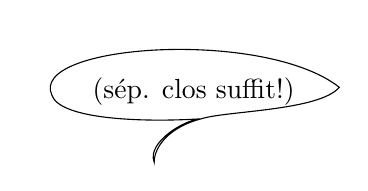
\begin{tikzpicture}[baseline=(m.base)]
\node[inner sep=2pt] (m) at (0,0) {(\uline{sép. clos suffit!})};
\draw (-1.8,-0.05)..controls(-2.1,0.6)and(0.9,0.8)..(1.85,0.05)..controls(1.6,-0.25)and(0.4,-0.25)..(0.1,-0.35)..controls(-0.3,-0.45)and(-0.5,-0.7)..(-0.5,-0.9)..controls(-0.6,-0.65)and(-0.1,-0.35)..(0.1,-0.35)..controls(-0.7,-0.4)and(-1.7,-0.35)..(-1.8,-0.05);
\end{tikzpicture}}}
$X$ propre sur $k$, $P/X$ loc de \deleted{présentation} \inserted{type} fini. Alors
$\displaystyle\prod_{X/k}P/X$ représentable par préschéma loc \unsure{algébrique}.
Si $P/X$ quasi-projectif, \inserted{ou seulement à fibres qu. pr.}
alors $\displaystyle\prod_{X/k}P/k$ est
essentiellement quasi-projectif [i.e. tout ouvert
quasi-compact est quasi-projectif] sur $k$.
\margin{\unsure{Il} suffit que pour $\forall\ x\in\operatorname{Ass}\underline{O}_X$,
$\exists\ y\in\bar x$ tel que la fibre $P_y$ soit quasi-projective.}
